\documentclass[a4paper]{article}

%% Language and font encodings
\usepackage[english]{babel}
\usepackage[utf8x]{inputenc}
\usepackage[T1]{fontenc}
\usepackage{amsmath}
\newcommand\norm[1]{\left\lVert#1\right\rVert}

%% Sets page size and margins
\usepackage[a4paper,top=3cm,bottom=2cm,left=3cm,right=3cm,marginparwidth=1.75cm]{geometry}

%% Useful packages
%%%%%%%%% begin snippet
%% You need to add the package "tabularx".
%% Place the snippet right after \begin{document}

% need tabularx
\usepackage{tabularx}
\usepackage{amsmath}
\usepackage{graphicx}
\usepackage[colorinlistoftodos]{todonotes}
\usepackage{paralist}
\usepackage{amssymb,amsmath,amsthm,enumitem}
\usepackage[colorlinks=true, allcolors=blue]{hyperref}
\usepackage{subcaption}
\setlength{\abovedisplayskip}{3pt}
\setlength{\belowdisplayskip}{3pt}
\usepackage[hypcap=false]{caption}

\captionsetup{justification=centering}
\captionsetup{format=plain, font=small, labelfont=bf}

\begin{document}
\title{ Computational Intelligence, SS2018 Assignment 3}

\begin{titlepage}
       \begin{center}
             \begin{huge}
				   %% Update assignment number here
                   \textbf{Assignment 3}
             \end{huge}
       \end{center}

       \begin{center}
             \begin{large}
                   Computational Intelligence, SS2018
             \end{large}
       \end{center}

       \begin{center}
 \begin{tabularx}{\textwidth}{|>{\hsize=.33\hsize}X|>{\hsize=.33\hsize}X|>{\hsize=.33\hsize}X|} 

                   \hline
                   \multicolumn{3}{|c|}{\textbf{Team Members}} \\
                   \hline
                   STRUGER & Patrick & 01530664 \\
                   \hline
                   B\"OCK & Manfred & 01530598 \\
                   \hline
                   HAUPT & Anna & 01432018 \\
                   \hline

             \end{tabularx}
       \end{center}

\end{titlepage}

%%%%%%%%% end snippet

\newpage
\tableofcontents
\newpage

\section{Linear SVM}
The file data.json contains the training set $(X, Y )$ of a binary classification problem with two input dimensions
($X$ is the set of 2-dimensional points, $Y$ are labels). Your task is to use a linear soft-margin SVM to solve this classification problem and to inspect how its parameter $C$, the positive cost factor that penalizes
misclassified training examples (slack variables), influences the decision boundary found by SVM.
In function $ex\_1$ in file svm\_main.py the data points are first loaded from the data file and plotted so that we can observe the structure of the data. Do the following:

\begin{enumerate}[label=(\alph*)]
\item Fill in function ex\_1\_a in file svm.py to train an SVM with a linear kernel with the provided training data $'x'$ and $'y'$. Plot the training points, decision boundary and support vectors using function plot\_svm\_decision\_boundary in file svm\_plot.py (passing in only $'x'~and~'y'$ as parameters $'x\_train'$ and $'y\_train'$).

\begin{figure}[htp]
\centering
\begin{minipage}{0.4\textwidth}
  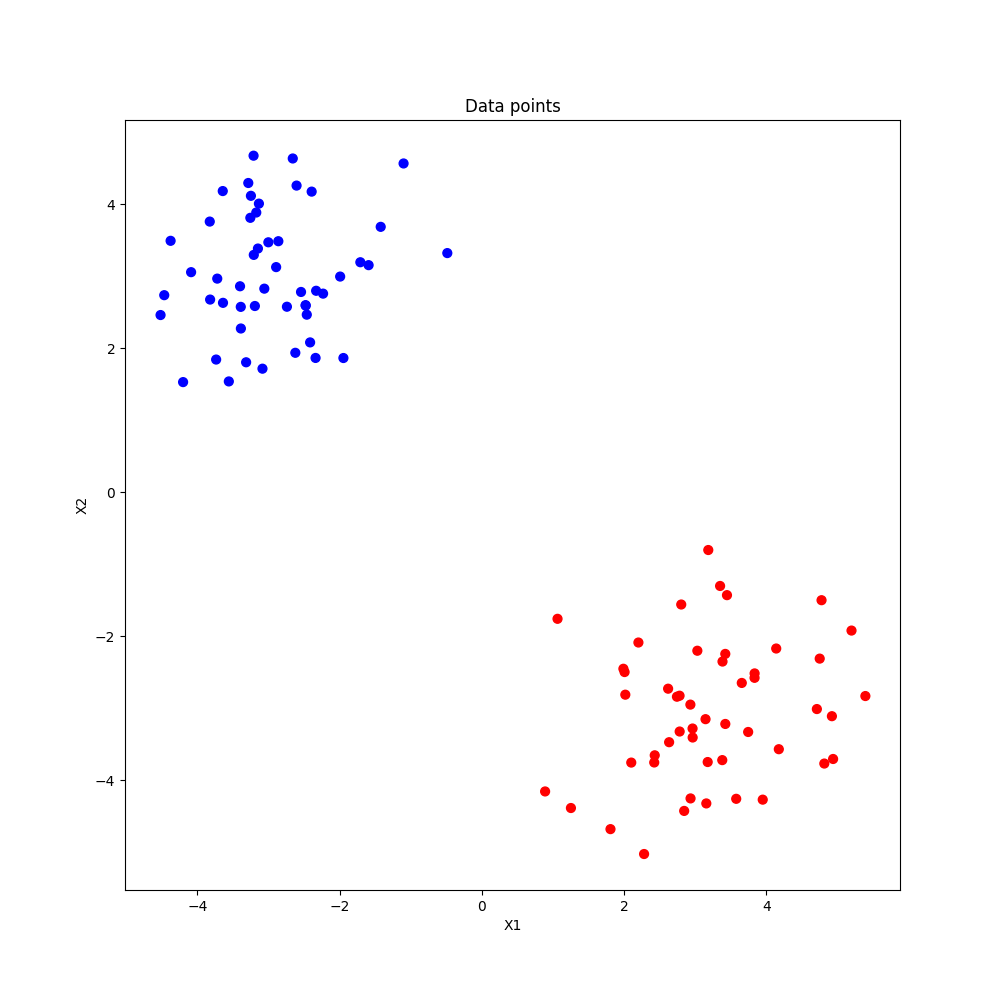
\includegraphics[scale=0.25]{plots/ex1.png}
  \captionof{figure}{Data structure of the data points.}
  \label{fig:1}
\end{minipage}
\hfill
\begin{minipage}{0.4\textwidth}
  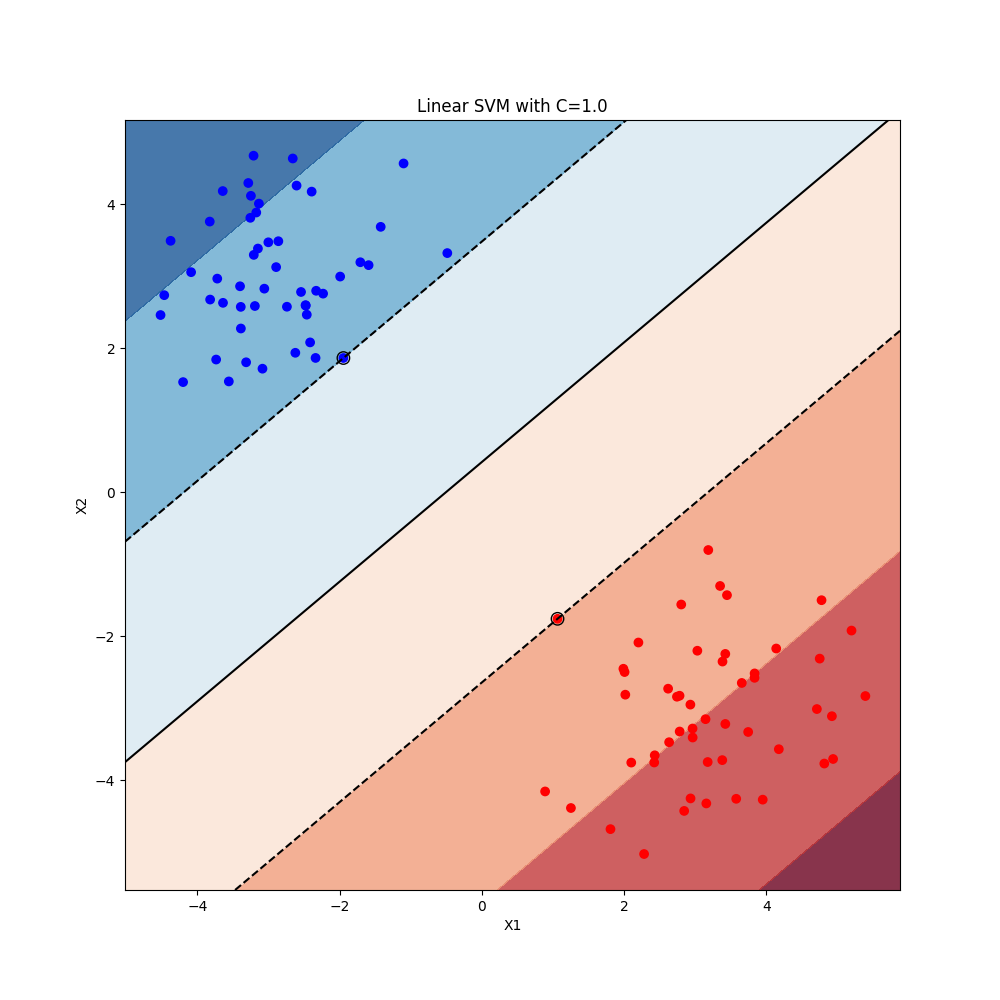
\includegraphics[scale=0.25]{plots/ex1a.png}
  \captionof{figure}{The decision boundary and support vectors.}
  \label{fig:2}
\end{minipage}
\end{figure}

\item In function ex\_1\_b in file svm.py add an additional data point (4,0) with label 1 to the data. Train a linear SVM again on this extended data. Plot results using plot\_svm\_decision\_boundary.

\begin{figure}[htp]
\centering
  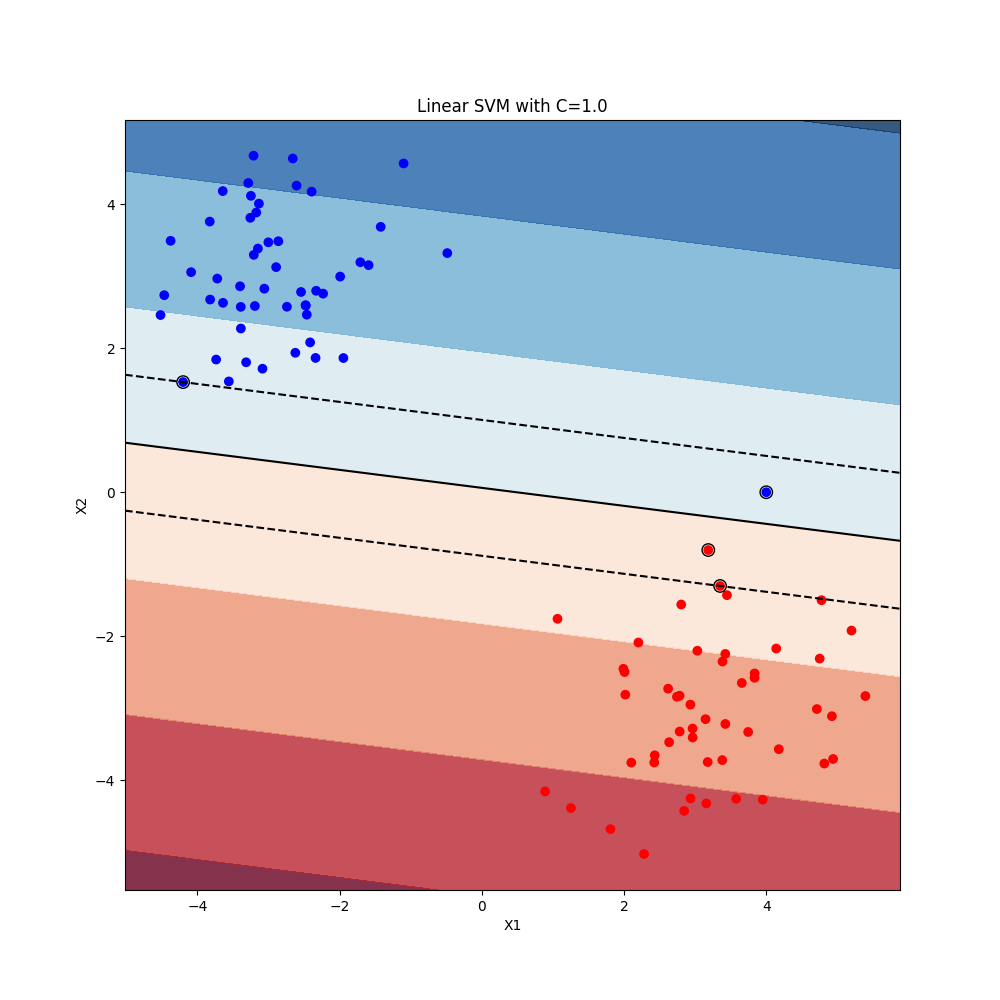
\includegraphics[scale=0.25]{plots/ex1b.png}
  \captionof{figure}{The decision boundary and support vectors after adding 	additional data point.}
  \label{fig:3}
\end{figure}

\textbf{For task b), discuss how and why the decision boundary changed when the new point was added.} \newline
After adding a new data point at \textit{(4, 0)} with \textit{label1} to the data set, the decision boundary gets more horizontal because the SVM tries to find a decision boundary to separate the classes best.

\newpage

\item In function ex\_1\_c in file svm.py, again extend the dataset as above, and train linear SVMs with different values of the parameter $C: 10^6,~10^0,~10^{−1}$, and $10^{−3}$. Plot the decision boundaries and support vectors for each of these values of $C$.

\begin{figure}[htp]
\centering
\begin{minipage}{0.4\textwidth}
  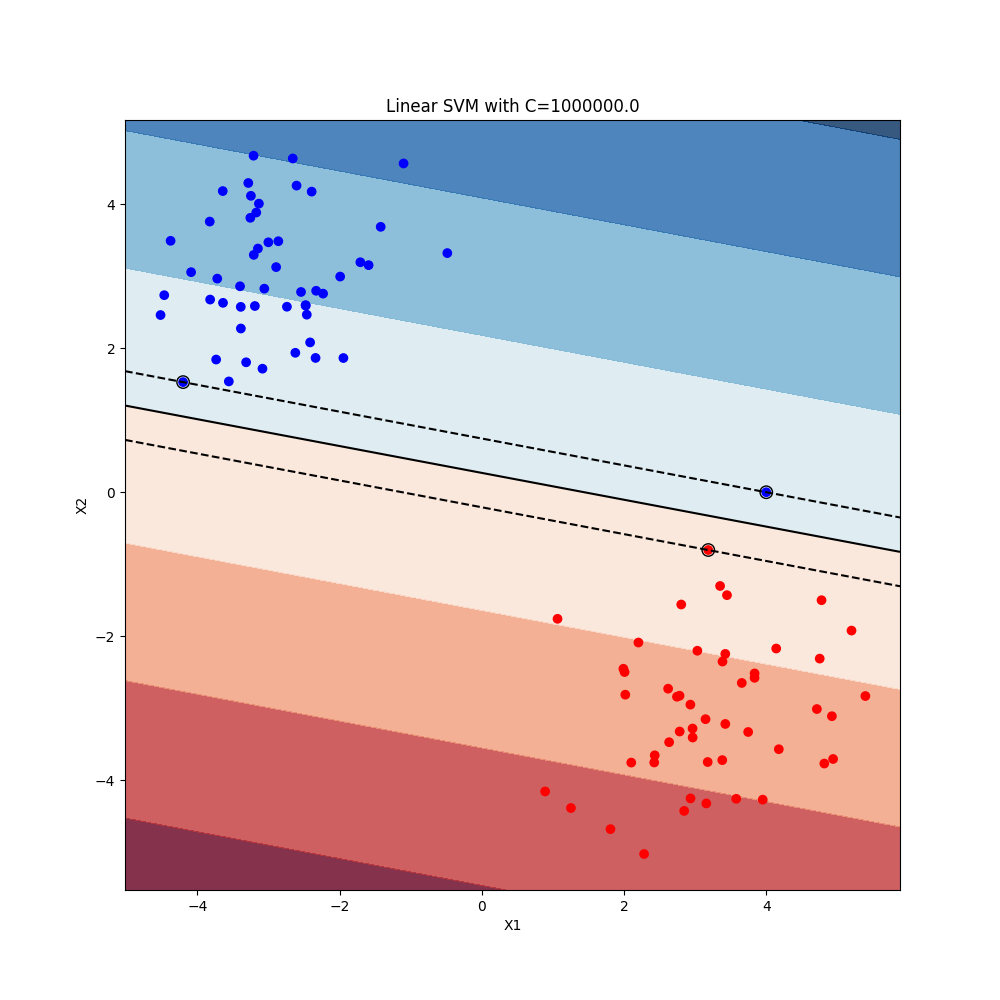
\includegraphics[scale=0.25]{plots/ex1c_1.png}
  \captionof{figure}{The decision boundary and support vectors with parameter \textit{$C = 10^6$}.}
  \label{fig:4}
\end{minipage}
\hfill
\begin{minipage}{0.4\textwidth}
  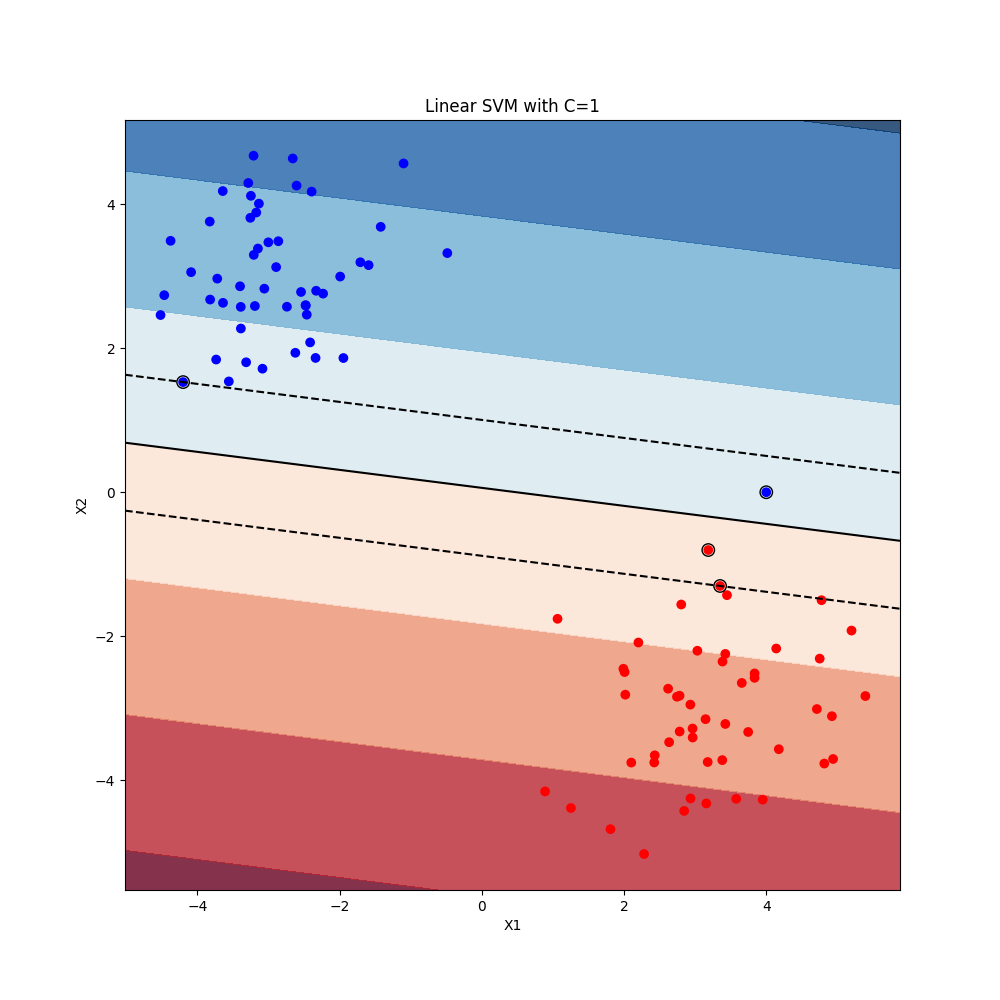
\includegraphics[scale=0.25]{plots/ex1c_2.png}
  \captionof{figure}{The decision boundary and support vectors with parameter \textit{$C = 10^0$}.}
  \label{fig:5}
\end{minipage}
\end{figure}

\begin{figure}[htp]
\centering
\begin{minipage}{0.4\textwidth}
  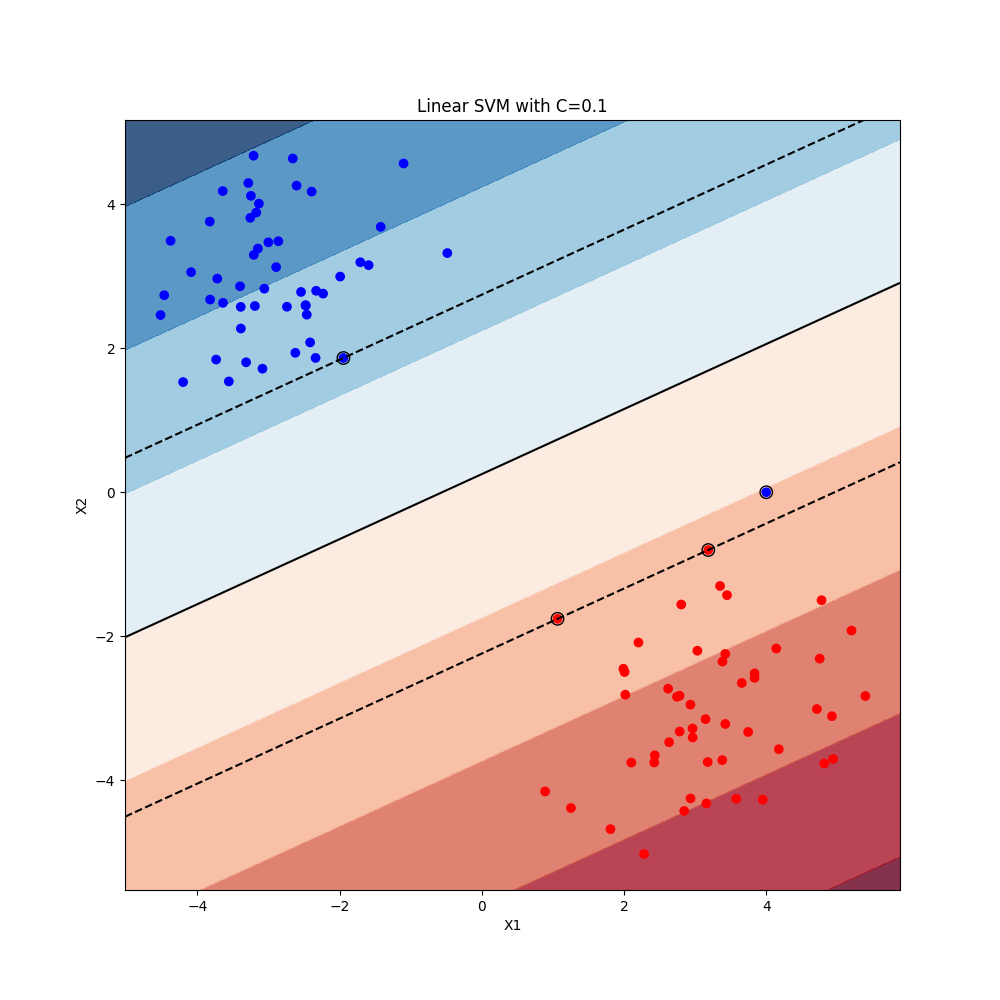
\includegraphics[scale=0.25]{plots/ex1c_3.png}
  \captionof{figure}{The decision boundary and support vectors with parameter \textit{$C = 10^{−1}$}.}
  \label{fig:6}
\end{minipage}
\hfill
\begin{minipage}{0.4\textwidth}
  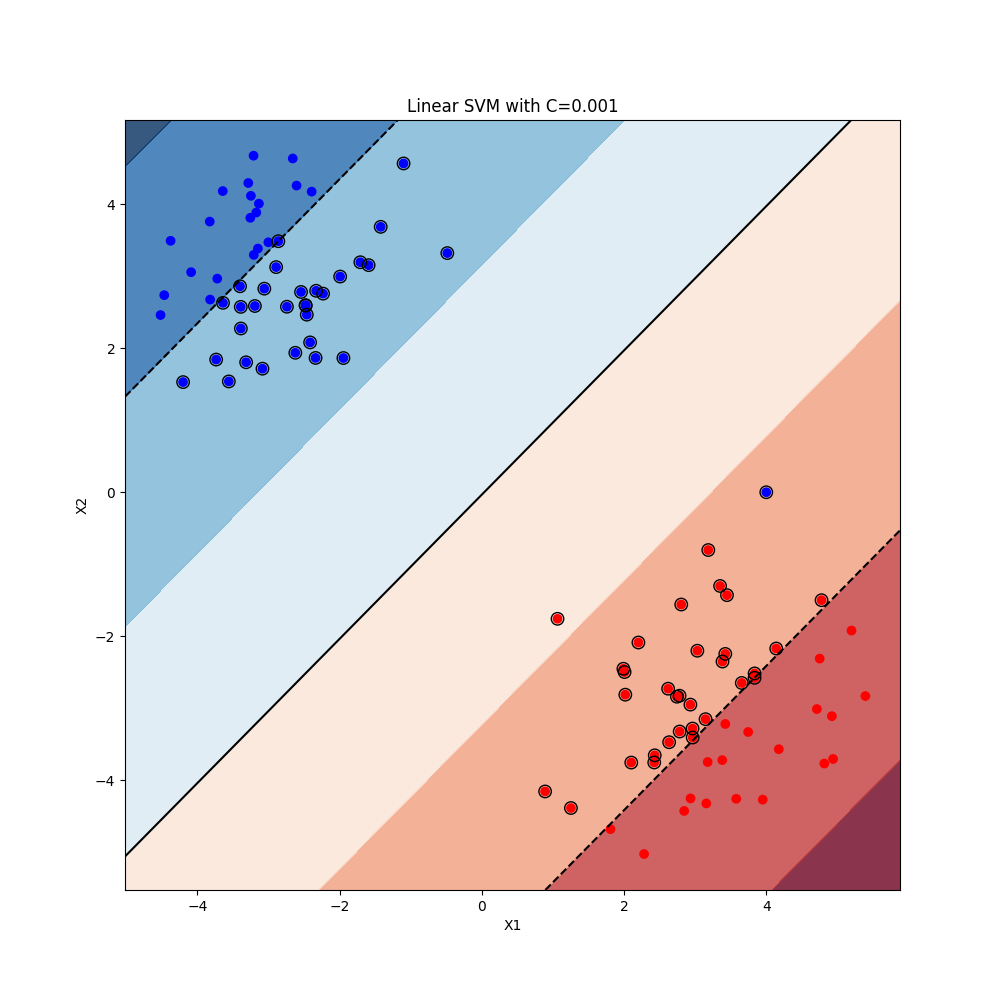
\includegraphics[scale=0.25]{plots/ex1c_4.png}
  \captionof{figure}{The decision boundary and support vectors with parameter \textit{$C = 10^{−3}$}.}
  \label{fig:7}
\end{minipage}
\end{figure}

\end{enumerate}

\textbf{For task c):}
\begin{itemize}
  \item \textbf{Report how the parameter $C$ influences the decision boundary found by the SVM.}
  By reducing the cost factor \textit{C}, the SVM tries to find decision boundaries where all data points of the same class are included. If the cost factor \textit{C} gets smaller, the SVM tries to focus on the main occurrence of a data point class. As shown in \ref{fig:7} the SVM focuses on the main occurrence of the red data points and ignores the additional blue one.
  
\item \textbf{How does the number of support vectors found by the SVM change with the value of $C$? Why?}
The number of support vectors decreases by an increase of the cost factor \textit{C}. If the value of \textit{C} increases, so the SVM tries to find a decision boundary to include data points of same class, which turns out that the support vectors are only the closest vectors to the decision boundary. While decreasing the cost factor \textit{C} the number of data points not belonging to the same class increases and so the number of support vectors increases as well.
\end{itemize}

\newpage

\section{Nonlinear (kernel) SVM}

The file data\_nl.json contains the training $(X, Y )$ and test $(XT, Y T)$ sets of a binary classification problem with two input dimensions. The goal of this task is to use different kernels (linear, polynomial and RBF) in combination with SVM in order to solve this nonlinear classification problem and to inspect the influence of kernel parameters on the classification error.

In function ex\_2 in file svm\_main.py the data points are first loaded from the data file and plotted so that we can observe the non-linear structure of the data (The training points are plotted in dark colors, and the testing points in lighter colors).\newline
We consider the following kernels:

\begin{itemize}
\item Linear kernel: $K(x, y) = x^T y$
\item Polynomial (non-homogeneous) kernel: $K(x, y) = (x^T y + r)^d$
\item RBF kernel: $ K(x, y) = exp(−\gamma\norm{x − y}^2)$ where $\gamma =\frac{1}{2\sigma^2}$
\end{itemize}
Do the following: \newline

\begin{enumerate}[label=(\alph*)]
\item Fill in function ex\_2\_a in file svm.py to train and test an SVM with a linear kernel with the provided training data \textit{'x\_train'} and \textit{'y\_train'}. Plot the training points, decision boundary and support vectors using function plot\_svm\_decision\_boundary in file svm\_plot.py. Calculate the test score.

\begin{figure}[htp]
\centering
\begin{minipage}{0.4\textwidth}
  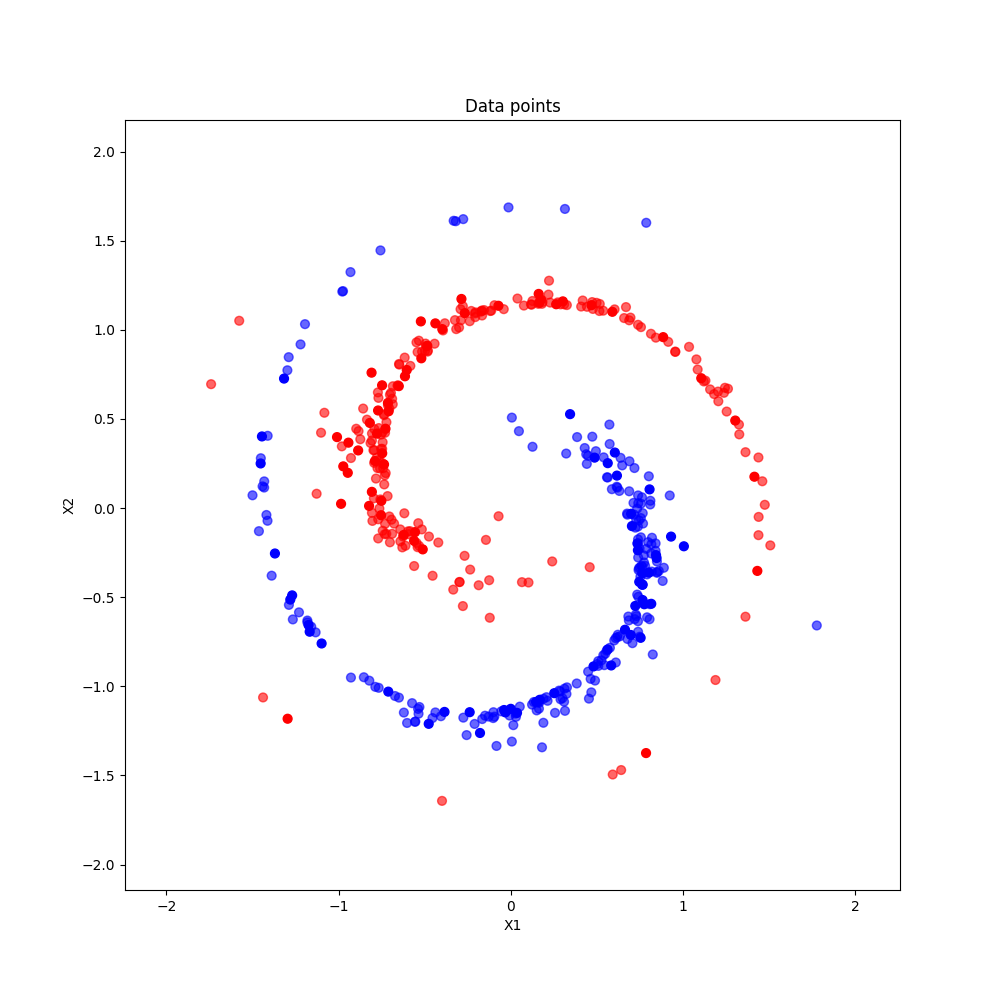
\includegraphics[scale=0.30]{plots/ex2.png}
  \captionof{figure}{Data structure of the data points.}
  \label{fig:8}
\end{minipage}
\hfill
\begin{minipage}{0.4\textwidth}
  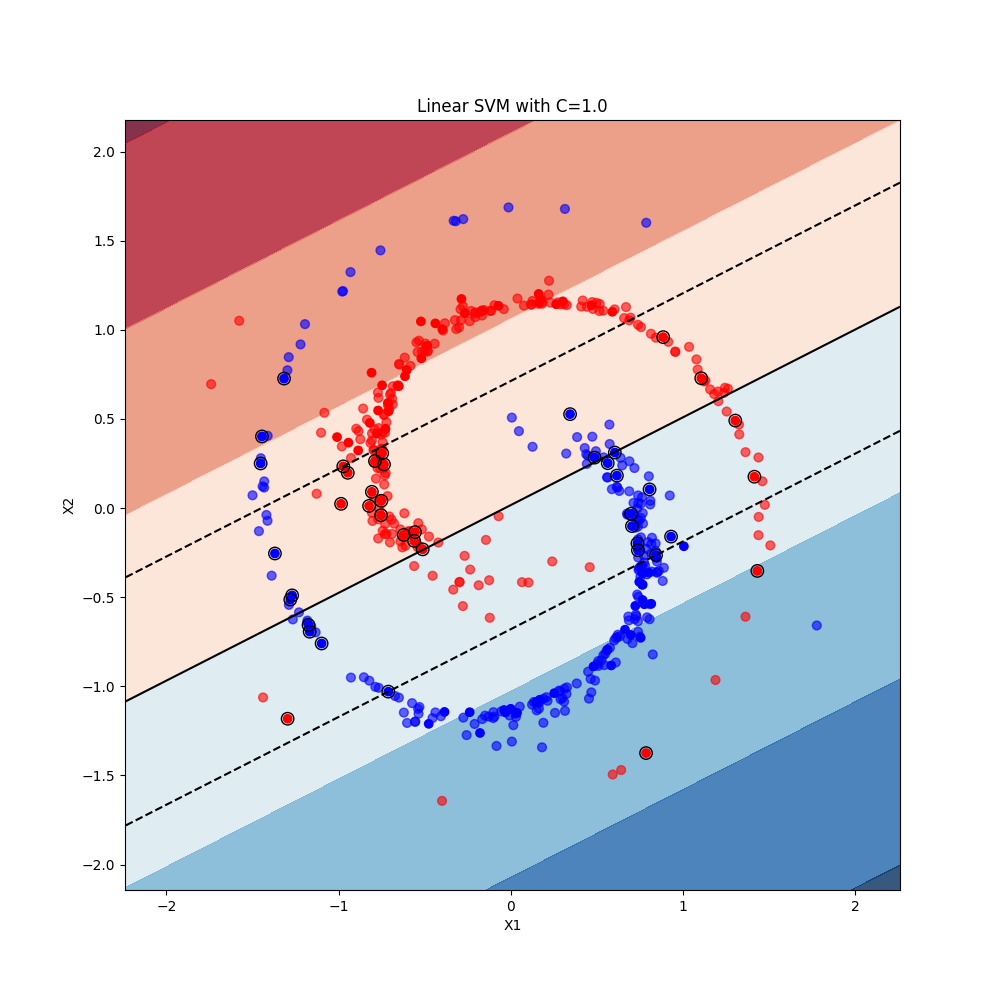
\includegraphics[scale=0.30]{plots/ex2a.png}
  \captionof{figure}{The training points, decision boundary and support vectors using linear kernel.}
  \label{fig:9}
\end{minipage}
\end{figure}

\newpage

\item In function ex\_2\_b in file svm.py train and test SVMs with a polynomial kernel for different degrees of the polynomial $d = 1, 2, . . . , 19, 20$ (Setting the value of r to 1). Plot the variation of training and testing score with polynomial degree using function plot\_score\_vs\_degree in file svm\_plot.py.
Plot the decision boundary and support vectors for the kernel with the highest test score using plot\_svm\_decision\_boundary. \newline \newline

\begin{figure}[htp]
\centering
\begin{minipage}{0.4\textwidth}
  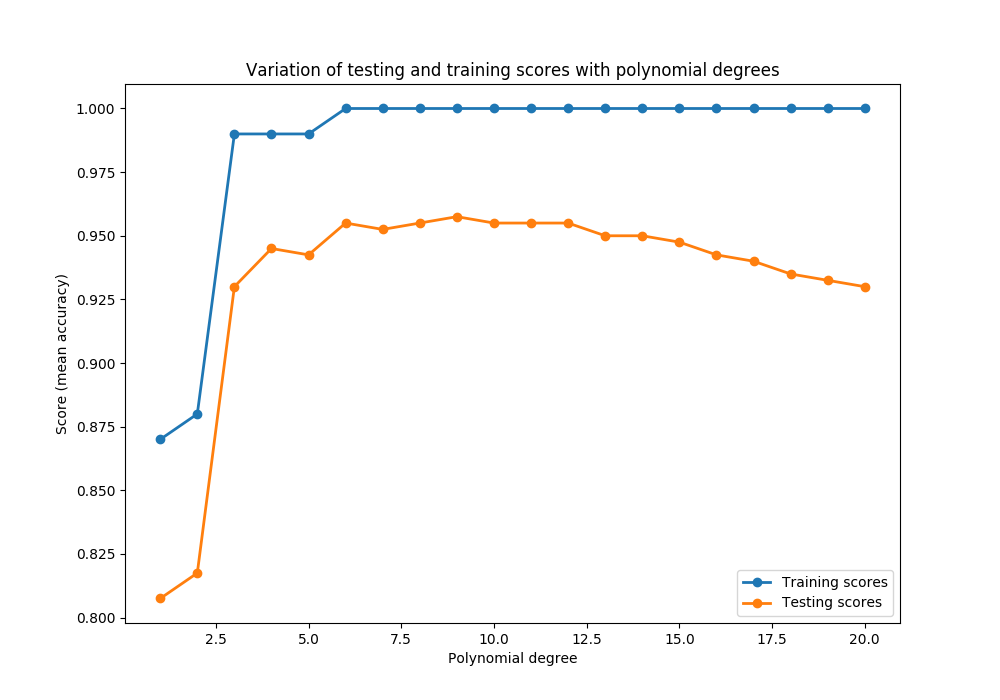
\includegraphics[scale=0.38]{plots/ex2b_1.png}
  \captionof{figure}{Variation of training and testing score with polynomial degree.}
  \label{fig:10}
\end{minipage}
\hfill
\begin{minipage}{0.4\textwidth}
  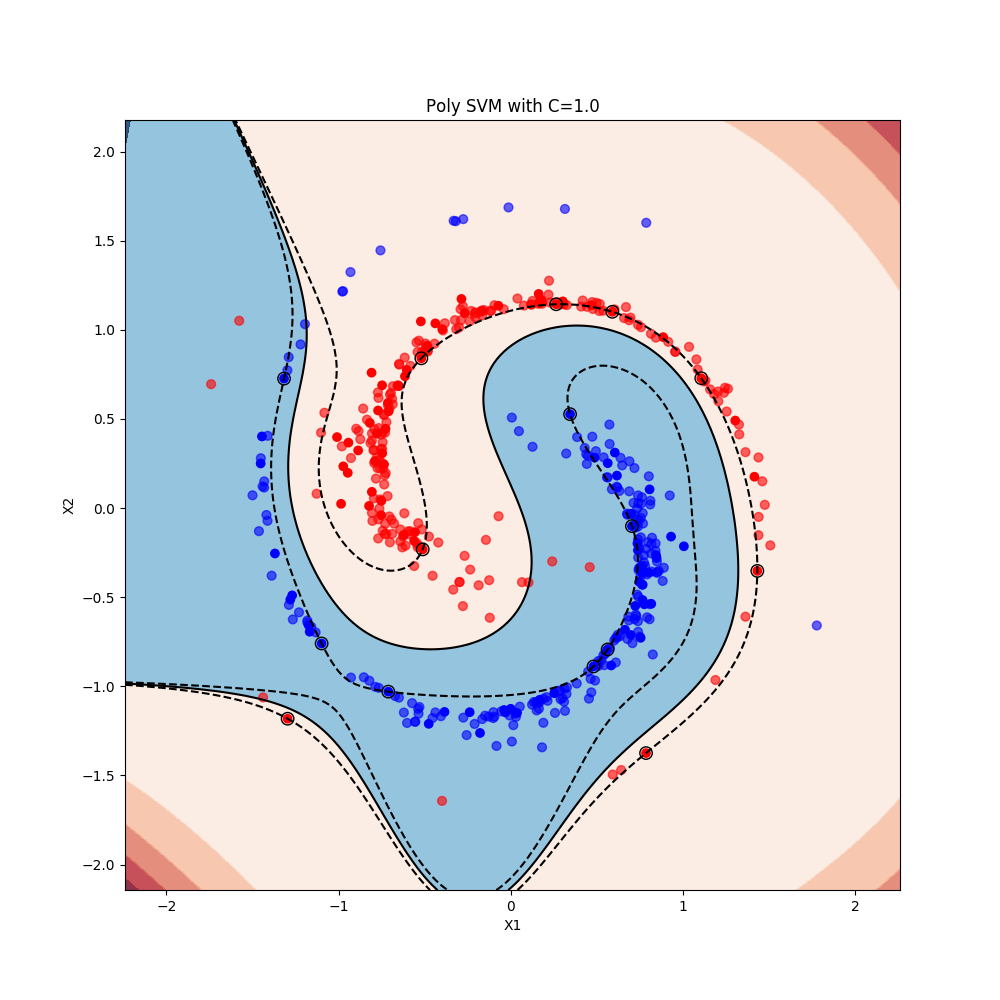
\includegraphics[scale=0.30]{plots/ex2b_2.png}
  \captionof{figure}{Decision boundary and support vectors for the kernel with the highest test score. \textcolor{red}{[ntbd]}}
  \label{fig:11}
\end{minipage}
\end{figure}

\textbf{For task b) which degree of the polynomial produces the highest test score (accuracy)? Report this
test score.} \newline
Degree 9 produces the Highest Test Score 0.9575

\newpage

\item Fill in function ex\_2\_c in file svm.py to repeat the above steps for an RBF kernel with values of $\gamma = 0.01, 0.03, . . . , 1.97, 1.99$. Plot the variation of training and testing score with the value of $\gamma$ using the function plot\_score\_vs\_gamma in file svm\_plot.py. Plot the decision boundary and support vectors for the kernel with the highest test score using plot\_svm\_decision\_boundary.
\newline \newline

\begin{figure}[htp]
\centering
\begin{minipage}{0.4\textwidth}
  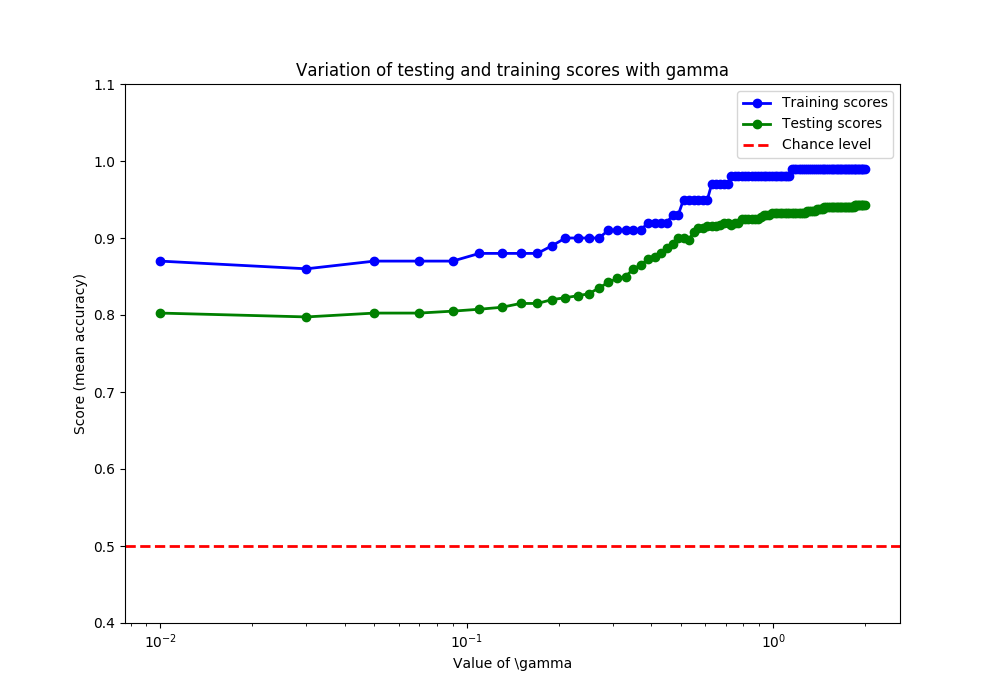
\includegraphics[scale=0.38]{plots/ex2c_1.png}
  \captionof{figure}{Variation of training and testing score with RBF kernel.}
  \label{fig:12}
\end{minipage}
\hfill
\begin{minipage}{0.4\textwidth}
  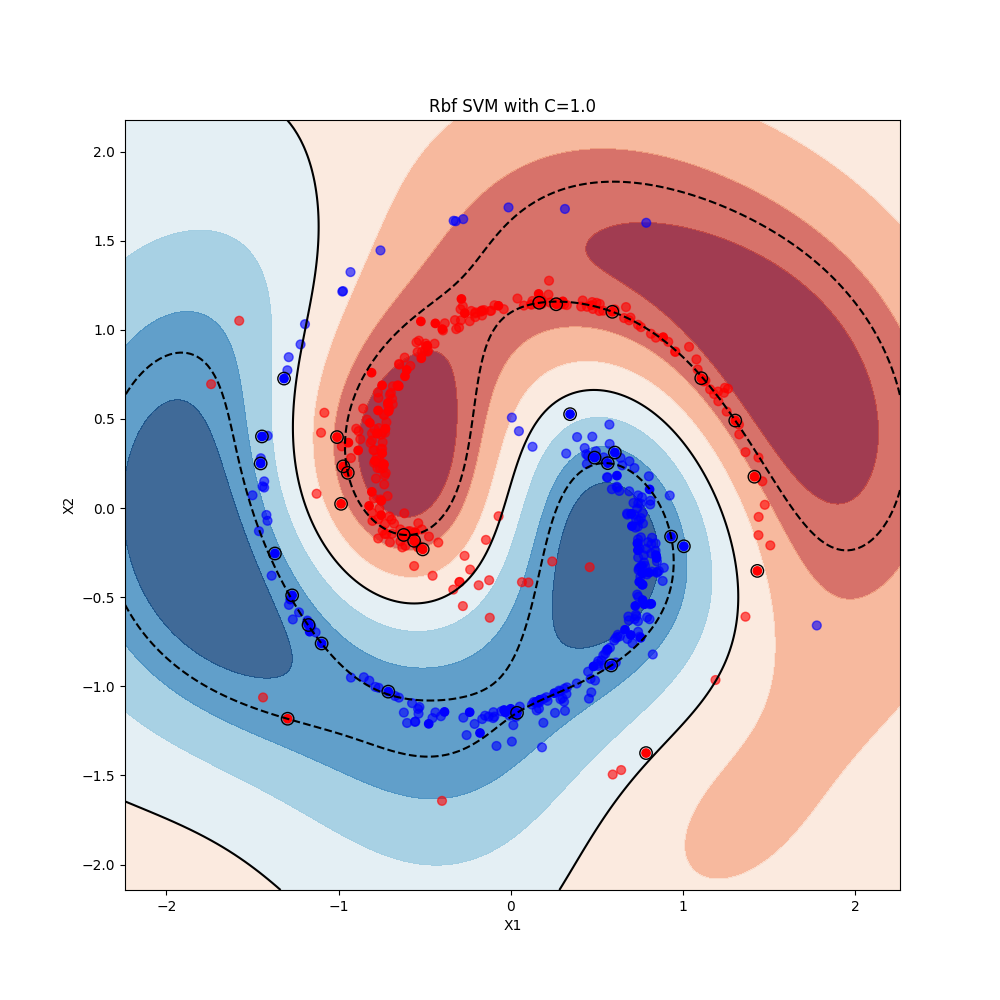
\includegraphics[scale=0.30]{plots/ex2c_2.png}
  \captionof{figure}{Decision boundary and support vectors for the kernel with the highest test score.}
  \label{fig:13}
\end{minipage}
\end{figure}

\begin{itemize}
\item \textbf{For task c) which value of gamma produces the highest test score (accuracy)? Report this test score.} \newline
A Gamma value of 1.85 produces the Highest Test Score 0.9425

\item \textbf{Compare results obtained by each of these three kernels:}
\begin{enumerate}
\item State the maximum test score achieved for each of these kernels and the kernel parameter for which that was achieved.
\begin{table}[htp]
\centering
\label{max_test_score}
\begin{tabular}{|c|c|c|}
\hline
\textbf{Kernel Type} & \multicolumn{1}{l|}{\textbf{Kernel Parameter}} & \textbf{kernel} \\ \hline
\textbf{linear}      & /                                              & 0.8125          \\ \hline
\textbf{poly}  & Degree: 9                                      & 0.9575          \\ \hline
\textbf{rbf}         & $\gamma$: 1.85                    & 0.9425          \\ \hline
\end{tabular}
\caption{Highest Test Score for different Kernel Types}
\end{table}
\item Which of the considered kernels performs best and why?\newline
Of the three kernel types, the kernel type \textit{poly} scored the highest score because \textcolor{red}{[ntbd]} it's logical 
\item Compare the complexity of decision boundaries and the number of Support Vectors found.\newline
 \textcolor{red}{[ntbd]}
\item Which kernel generalizes best for the given dataset?\newline
For the given dataset the poly Kernel generalizes best
\textcolor{red}{[ntbd]}
\end{enumerate}
\end{itemize}

\end{enumerate}

\newpage
\section{Multiclass classification}
For this task you will use a linear SVM as a binary classifier to solve a multiclass problem. For this purpose use the data file data\_mnist.json which contains training $(X, Y )$ and test $(XT, Y T)$ sets of handwritten digits. To simplify the problem we consider only the first $5$ digits: $1, . . . , 5$. Each data sample in $X$ (a handwritten digit) is an image of $28 \times 28$ pixels. Note that here the labels are not binary, but rather each data sample belongs to one of the $5$ classes. Load the data file and plot several data samples to see handwritten digits (use plot\_mnist). The goal of this task is to use the one-vs-all approach with SVM for multiclass classification in order to recognize digits. In all simulations of this task use the parameter $C = 10$. 
In function ex\_3 in file svm\_main.py the data points are first loaded from the data file and plotted so that we can observe the structure of the MNIST dataset. Do the following:
\begin{enumerate}[label=(\alph*)]
\item In function ex\_3\_a in the file svm.py, use the scikit learn implementation of one-versus-rest multiclass classification. This is done by specifying the argument $decision\_function\_shape='ovr'$ when creating the classifier object. Train the classifier on the MNIST dataset for a LINEAR kernel and a RBF kernel with gamma ranging from $10^5$ to $10^{−5}$ (plot this for $10$ values of gammas in between). Plot the results with plot\_score\_vs\_gamma, and specify the score obtained with a linear kernel using the optional argument lin\_score\_train. Note that the chance level has changed for this example.
\item In function ex\_3\_b in the file svm.py, train a multi-class SVC with a linear kernel. Use the function confusion\_matrix from scikit-learn to get the confusion matrix. Plot the confusion matrix with plot\_confusion\_matrix. Plot the first $10$ images from the test set of the most misclassified digit using plot\_mnist. (For example, if digit 3 is the most misclassified digit, plot the first $10$ images miss-classified as 3 in the test set)

\end{enumerate}
In your report:
\begin{itemize}
\item Recall the algorithms ‘One-versus-Rest’ (or versus-all) and ‘One-versus-one’ multi-class classification
procedures. How many binary classifiers need to be trained in both cases?
\item Include plots for ex\_3\_a with the scores of a linear and a rbf kernels.
\item Discuss those results. In particular why does a linear kernel perform well on images?
\item Find the digit class for which you get the highest error rate.
\item Include plots for ex\_3\_b of the confusion matrix and the first $10$ images from the test set of the most misclassified digit.
\item With the help of these two plots, discuss why the classifier is doing these mistakes.
\end{itemize}

\end{document}




